\documentclass[border=10pt]{standalone}
\usepackage{tikz}\usepackage{amsmath}\usetikzlibrary{calc,arrows.meta}
\begin{document}
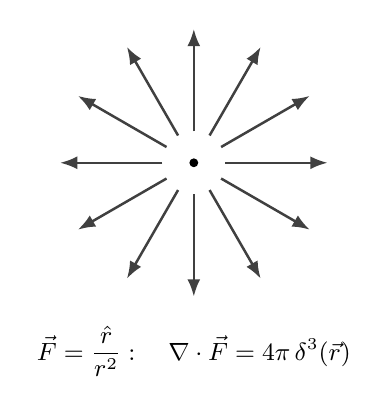
\begin{tikzpicture}[line width=0.9pt,>={Latex[length=2.2mm]}]
  \fill (0,0) circle(1.6pt);
  \foreach \a in {0,30,...,330} \draw[->,black!75] (\a:0.4)--(\a:1.7);
  \node at (0,-2.4){\small $\vec F=\dfrac{\hat r}{r^2}:\quad \nabla\cdot\vec F=4\pi\,\delta^3(\vec r)$};
\end{tikzpicture}
\end{document}
